
\medskip

Heiata et Hiro ont choisi comme gâteau de mariage une pièce montée composée de 3 gâteaux cylindriques superposés, tous centrés sur l'axe (d) comme l'indique la figure ci-dessous :

\medskip
 
\parbox{0.4\linewidth}{

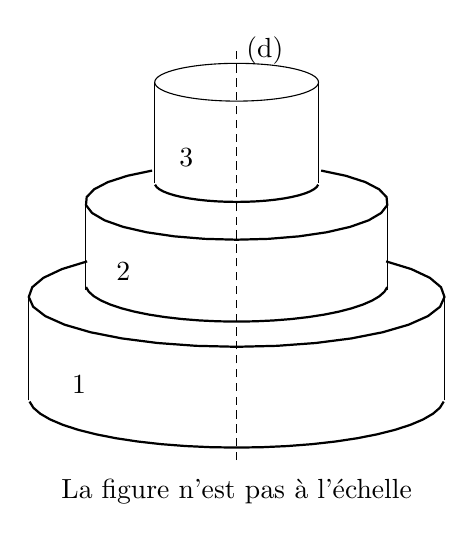
\begin{tikzpicture}[x=0.8cm, y=0.8cm]

% Ellipses
\draw[line width=0.8pt, domain=-5:-175] plot ({3.3*cos(\x)}, {2 + 0.8*sin(\x)});
\draw[line width=0.8pt, domain=44:-224]  plot ({3.3*cos(\x)}, {3.6 + 0.8*sin(\x)});
\draw[line width=0.8pt, domain=-5:-175]  plot ({2.4*cos(\x)}, {3.8 + 0.6*sin(\x)});
\draw[line width=0.8pt, domain=56:-236]  plot ({2.4*cos(\x)}, {5.1 + 0.6*sin(\x)});
\draw[line width=0.8pt, domain=-5:-175]  plot ({1.3*cos(\x)}, {5.4 + 0.3*sin(\x)});

% Ellipse complète du haut
\draw (0,7) ellipse [x radius=1.3, y radius=0.3];

% Traits verticaux
\draw (-1.3,5.4) -- (-1.3,7);
\draw (1.3,5.4) -- (1.3,7);
\draw (-2.4,3.7) -- (-2.4,5.1);
\draw (2.4,3.7) -- (2.4,5.1);
\draw (-3.3,1.95) -- (-3.3,3.57);
\draw (3.3,1.95) -- (3.3,3.57);

% Axe vertical pointillé
\draw[densely dashed, line width=0.2pt] (0,1) -- (0,7.5);

% Texte
\node[anchor=west] at (0,7.5) {(d)};
\node at (0,0.5) {La figure n'est pas à l'échelle};
\node at (-2.5,2.2) {\no 1};
\node at (-1.8,4)   {\no 2};
\node at (-0.8,5.8) {\no 3};

\end{tikzpicture}}\hfill
\parbox{0.55\linewidth}{
\begin{itemize}
\item[$\bullet~~$] Les trois gâteaux cylindriques sont de même hauteur : 10 cm. 
\item[$\bullet~~$] Le plus grand gâteau cylindrique, le \no 1, a pour rayon 30 cm. 
\item[$\bullet~~$] Le rayon du gâteau \no 2 est égal au $\frac{2}{3}$ de  
celui du gâteau \no 1. 
\item[$\bullet~~$] Le rayon du gâteau \no 3 est égal au $\frac{3}{4}$ de  celui du gâteau \no 2.
\end{itemize}}

\medskip 
	 	 
\begin{enumerate}
\item Montrer que le rayon du gâteau \no 2 est de $20$~cm. 
\item Calculer le rayon du gâteau \no 3. 
\item Montrer que le volume total \textbf{exact} de la pièce montée est égal à \np{15250}$\pi$ cm$^3$.
 
Rappel :  le volume $V$ d'un cylindre de rayon $R$ et de hauteur $h$ est donné par la formule  $V = \pi \times R^2 \times h$. 
\item Quelle fraction du volume total représente le volume du gâteau \no 2 ? Donner le résultat sous forme de fraction irréductible. 
\end{enumerate}

\bigskip

